Z racji na to, że korzystamy z $m$ węzłów obliczeniowych typu homogenicznego, gdzie każdy węzeł posiada $k$ rdzeni,
siatkę podzieloną na $m \cdot k$ części należy podzielić na $m$ obszarów, każdy składający się
z $k$ podobszarów.
Bardzo ważną obserwacją jest, że w przeciwieństwie do poprzedniej części partycjonowania grafu na $m \cdot k$ części,
gdzie dopuszczalne były nierówności w kwestii pól pomiędzy obszarami, tutaj bardzo ważne jest aby każdy obszar składał
się z takiej samej liczby podobszarów.
Jest to poważne utrudnienie tego problemu.

\begin{figure}[h]
\centering
\begin{subfigure}{.5\textwidth}
    \centering
    \fbox{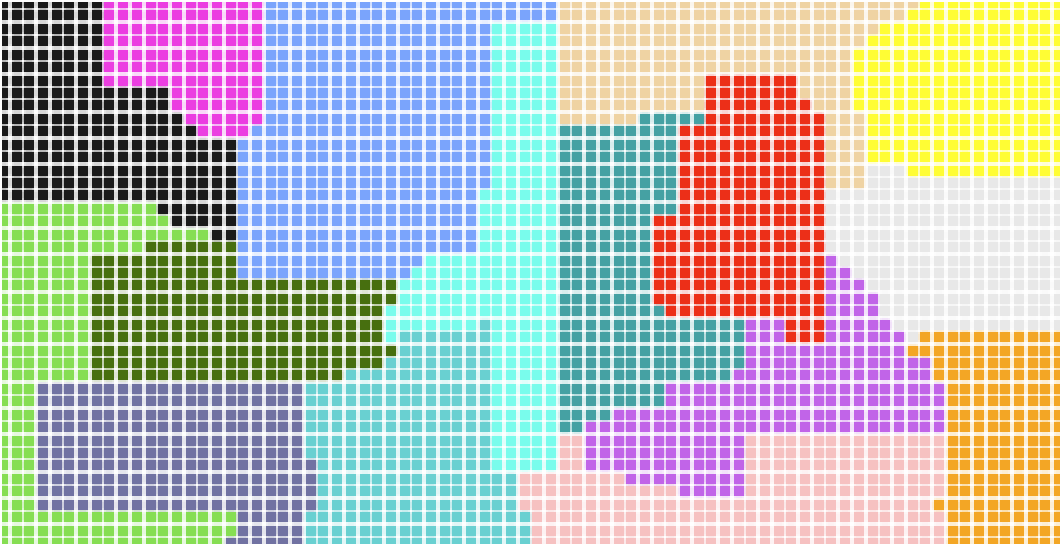
\includegraphics[width=0.8\textwidth]{images/m/1}}
    \caption[short]{}
\end{subfigure}%
\begin{subfigure}{.5\textwidth}
    \centering
    \fbox{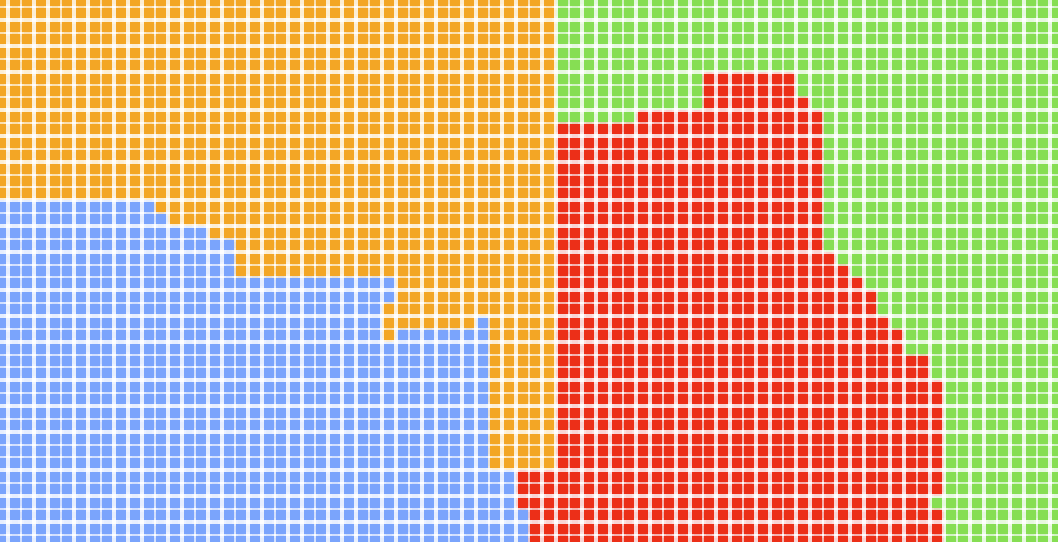
\includegraphics[width=0.8\textwidth]{images/m/2}}
    \caption[short]{}
\end{subfigure}
\caption{Obrazek (a) podział na $m \cdot k$ obszarów. Obrazek (b) przedstawia podział $m \cdot k$ obszarów na $m$ obszarów
po $k$ podobszarów. $m=4$ oraz $k=4$.}
\label{im:k_m}
\end{figure}

Ta część algorytmu jest realizowana przez algorytm weighted matching z dodatkiem części zachłannej.
Daną wejściową do algorytmu jest siatka z podziałem na $m \cdot k$ obszarów, jak na rysunku \ref{im:k_m}(a).
Najpierw wszystkie partycje redukowane są do pojedynczych wierzchołków.
Oznacza to, że mamy $m \cdot k$ wierzchołków.
Następnie graf składający się z $m \cdot k$ wierzchołków redukowany jest do $m$ wierzchołków
za pomocą algorytmu weighted matching, identycznego jak na rysunku \ref{code:lam}.
Po zredukowaniu do $m$ wierzchołków, do każdego wierzchołka przypisywana jest inna partycja.
Następnie graf jest odtwarzany z powrotem do rozmiaru $m \cdot k$ z zachowaniem nowych partycji.
W tym momencie otrzymujemy podział $m \cdot k$ wierzchołków na $m$ obszarów.

Charakterystyką algorytmu weighted matching jest to, że od idealnie równych podziałów bardziej ceni sobie obszary
''zbite'', czyli takie, które mają możliwie krótkie granice między sobą.
Jest to wpisane w jego charakterystykę na tyle mocno, że nie sposób tego zmienić.
W związku z powyższym w większości podziałów nie kończymy z podziałem $m$ obszarów po $k$ podobszarów każdy, tylko z czymś gorzej
podzielonym, natomiast całkiem bliskim podziałowi $m$ obszarów po $k$ podobszarów, bo choć LAM nie gwarantuje
nam podziałów idealnie równych,
to gwarantuje nam obszary o zbliżonej liczbie wierzchołków.

Czasami na tym etapie mamy już $m$ obszarów po $k$ podobszarów każdy.
Jeśli tak nie jest, to uruchamiana jest
zachłanna część algorytmu, która wyrównuje liczbę podobszarów pomiędzy obszarami.
Składa się ona z dwóch części.
Najpierw algorytm sprawdza jakie obszary leżą obok siebie i wyrównuje pola sąsiadów.
Przykładowo, jeśli leżą obok siebie dwa obszary $A$ oraz $B$, z czego $A$ zawiera $k-1$ podobszarów, natomiast $B$ $k+1$
podobszarów, to jeden z podobszarów graniczych przenoszony jest z $B$ do $A$ w celu wyrównania liczby
podobszarów do $k$ dla każdego z nich.
Jeśli $B$ zawierałby $k+3$ obszary, natomiast A $k-1$, to z $B$ przeniesiony zostaną dwa obszary do $A$.
W ten sposób podobszary z dużych obszarów mają sposobność ''rozproszyć'' się po siatce.
W kolejnej turze nadmiarowe obszary z $A$ mają szansę zostać przeniesione gdzie indziej.
Ta część algorytmu wywoływana jest dopóki nie przestanie przynosić nowych zmian.
Ponieważ operujemy na wierzchołkach, które mają duże wagi to już na tym etapie przesunięcia obszarów powodują często
tworzenie się obszarów dwuczęściowych.

Jeśli po tym etapie nadal nie mamy równych obszarów następuje ostatni etap algorytmu.
Ten etap działa dopóki wszystkie obszary nie będą miały takiej samej liczby wierzchołków.
Wybierany jest zawsze obszar o największej i najmniejszej liczbie podobszarów.
Następnie z obszaru o większej liczbie podobszarów losowne są podobszary, a następnie przenoszone do
obszaru o mniejszej liczbie podobszarów dopóki wybrana para obszarów nie będzie miała równego rozmiaru.

Zaletą tego algorytmu jest niski koszt obliczeniowy oraz prostota, im bardziej udany podział z algorytmu
weighted matching tym wieksza szansa na dobry podział końcowy.
Liczby wierzchołków, na których operuje algorytm są bardzo małe więc można nawet wielokrotnie
wywoływać cały algorytm w poszukiwaniu najlepszego rezultatu.
Zaleta jest jednocześnie jego wadą, prostota algorytmu oraz jego zachłanna charakterystyka sprawia, że
jakość podziałów pod względem kryterium długości granic nie jest najwyższa - rysunek \ref{im:k_m2}.

\begin{figure}[h]
\centering
\begin{subfigure}{.5\textwidth}
    \centering
    \fbox{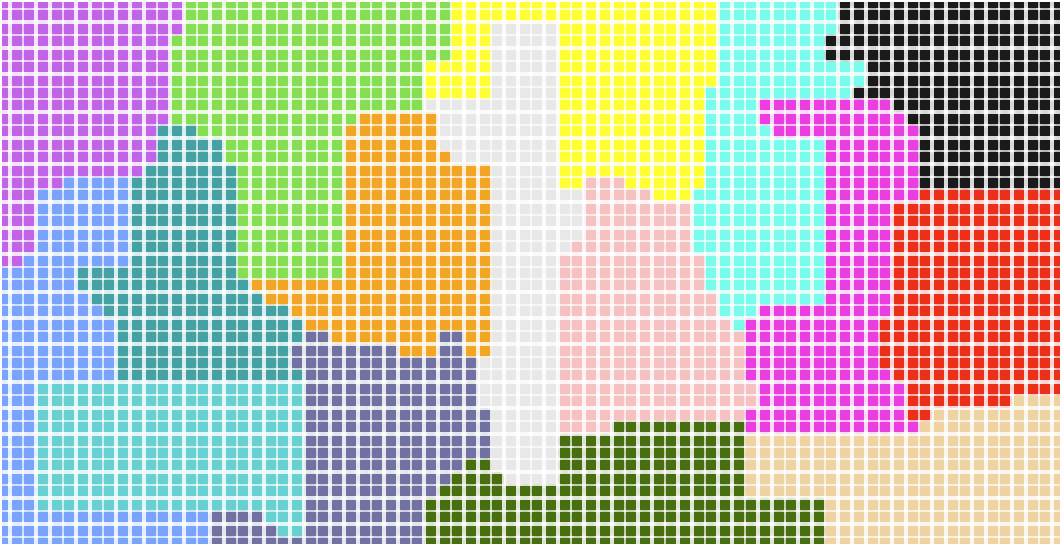
\includegraphics[width=0.8\textwidth]{images/m/3}}
    \caption[short]{}
\end{subfigure}%
\begin{subfigure}{.5\textwidth}
    \centering
    \fbox{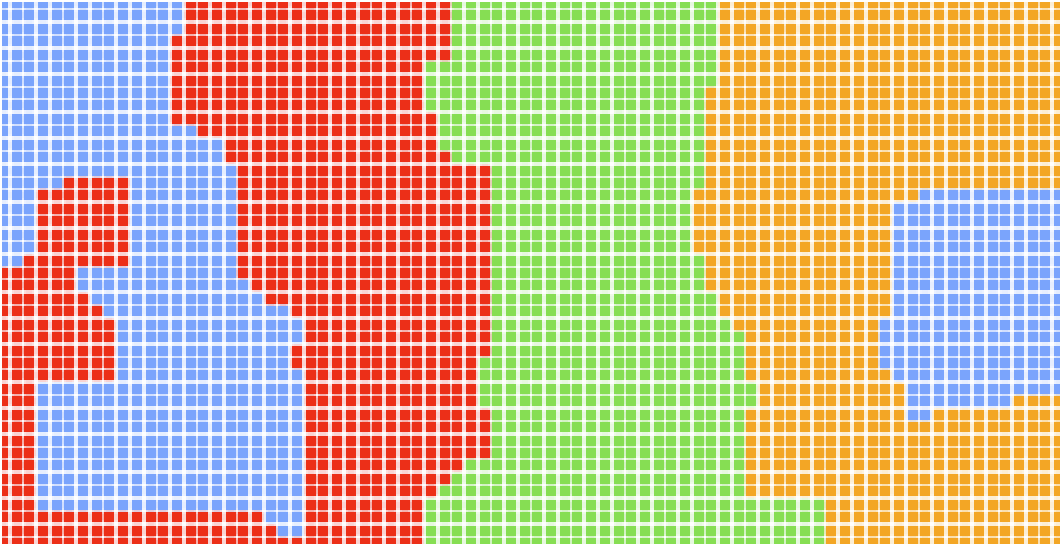
\includegraphics[width=0.8\textwidth]{images/m/4}}
    \caption[short]{}
\end{subfigure}
\caption{Obrazek (a) podział na $m \cdot k$ obszarów. Obrazek (b) przedstawia podział $m \cdot k$ obszarów na $m$ obszarów
po $k$ podobszarów. $m=4$ oraz $k=4$.}
\label{im:k_m2}
\end{figure}